\documentclass[conf]{new-aiaa}
%\documentclass[journal]{new-aiaa} for journal papers
\usepackage[utf8]{inputenc}

% template packages
\usepackage{graphicx}
\usepackage{amsmath}
\usepackage[version=4]{mhchem}
\usepackage{siunitx}
\usepackage{longtable,tabularx}
\setlength\LTleft{0pt} 

% graphics packages
% \usepackage{graphicx}

% algorithm packages
\usepackage{algpseudocode}
\usepackage{algorithm}
\usepackage{amsmath}

% symbols
\usepackage{gensymb}

% reference packages
\usepackage{cleveref}

% formatting packages
% \usepackage[parfill]{parskip}
% \setlength{\parindent}{0cm}
% \usepackage[margin=1in]{geometry}
\usepackage{subfigure}

% editing packages
\usepackage{todonotes}

\title{LES Validation of Wind Farm Layout Optimization Using a Simple Wake Model and Gradient-based Optimization}

\author{Jared J. Thomas\footnote{PhD Student, Department of Mechanical Engineering, 360 EB, Provo, UT 84602, AIAA Student Member}}
\affil{Brigham Young University, Provo, UT 84602}
\author{Jennifer Annoni \footnote{Research Engineer, National Wind Technology Center, 15013 Denver W Pkwy, Golden, CO 80401.}}
\author{Paul Fleming \footnote{Senior Engineer, National Wind Technology Center, 15013 Denver W Pkwy, Golden, CO 80401.}}
\affil{National Renewable Energy Laboratory, Golden, CO, 80401, USA}
\author{Andrew Ning\footnote{Assistant Professor, Department of Mechanical Engineering, 360 EB, Provo, UT 84602, AIAA Senior Member}}
\affil{Brigham Young University, Provo, UT 84602}

\begin{document}

\maketitle

% \begin{abstract}
% These instructions give you guidelines for preparing papers for AIAA Technical Papers using \LaTeX{}. Define all symbols used in the abstract. Do not cite references in the abstract. The footnote on the first page should list the Job Title and AIAA Member Grade for each author, if known Authors do not have to be AIAA members.
% \end{abstract}


\section{Introduction}
The Wind Farm Layout Optimization Problem (WFLOP) has been extensively studied in the literature \cite{samorani2013,lackner2007,parada2017,elkinton2008,tingey2015,thomas2015_sustech,valverde2014,fleming2015}. However, there is still significant progress that needs to be made before wind farms can be designed with the most efficient layouts. 
%For an extensive review of the area, refer to Herbert-Acero et al. (2014) \cite{acero2014}. 
One of the great hurdles to efficient wind farm layout design has been that the traditional optimization approach for wind farms, gradient-free optimization methods, does not scale well with large wind farms. Generally, gradient-free optimization methods are limited to relatively few variables and constraints \todo{citation}. The WFLOPs of interest often have hundreds to thousands of variables and constraints, exceeding the abilities of gradient-free optimization methods \todo{citation}.

To overcome the limits of gradient-free optimization, gradient-based methods can be used since they are well suited to problems with many variables and constraints. However, gradient-based methods are prone to premature convergence when used with multi-modal problems, such as the WFLOP \cite{acero2014}. Because of this weakness, gradient-based optimization methods have been ignored until recently. However, recent studies have demonstrated that significant improvements to wind farm layouts, if not global optimality, can be obtained through using gradient-based methods either alone \cite{fleming2015, gebraad2017-max-aep, thomas2017}\todo{cite WEC} or in a hybrid approach with gradient-free methods \cite{rethore2014}. However, large-scale gradient-based optimization results have yet to be validated with the more detailed simulation methods such as Large Eddy Simulation (LES). Such validation is critical for proving the benefits obtained through optimization methods are realistic, and not just an artifact of the simplified models being used. \todo{discuss limits of LES and how it is still useful}\todo{need a bridge to next paragraph}

Solving a WFLOP requires several different types of models. Two of the most important of these are the wake model and the farm model. Generally speaking, wind turbine wake models define the wind speed in a turbine wake given a set of inflow conditions, while farm models combine the wakes of various turbines to determine the cumulative effects of the wakes of multiple turbines. Many different wind turbine wake and wind farm models have been presented, all with varying levels of accuracy and computational cost. Many of the wake models, such as the Jensen/Park model \cite{jensen1983}, the Frandsen model \cite{frandsen2006}, and the original FLORIS model \cite{gebraad2014} have regions of non-physical zero-valued gradients, where their gradients go to zero while the gradients of the real design space do not. If a model with non-physical zero-valued gradients is used with gradient-based optimization, the optimization may converge to a very poor local optimum \cite{thomas2017}.

The Bastankhah and Port\'{e}-Agel wake model presented in \cite{bastankhah2014, bastankhah2016} is well suited to gradient-based optimization, with the exception of the near wake region, which is ignored in the model. The near wake region is rarely needed for evaluating a wind farm since wind turbines are usually placed far enough from each other that they are in the far wake. However, it is important to have the near wake region defined during gradient-based optimization because optimization algorithms may attempt infeasible solutions during the optimization process \cite{belegundu2011}. \todo{what is new}The new wake model uses a Gaussian distribution to define the wake, and is easily applied to different turbines since it only has one independent parameter. Building on this new \todo{new?} wake model, Niayifar and Port\'{e}-Agel have proposed a farm model \todo{check about one param (no params?)} \cite{niayifar2015, niayifar2016} to be used in concert with the Bastankhah and Port\'{e}-Agel wake model as published in 2014 \cite{bastankhah2014}, but a new version of the wake model was published in 2016 \cite{bastankhah2016}. There are some minor problems with the farm model in \cite{niayifar2016} for use with gradient-based optimization that need to be addressed.

In this work, we address the lack of near wake definition in the Bastankhah and Port\'{e}-Agel wake model for the purposes of using gradient-based optimization methods to solve the WFLOP. We then apply the Niayifar and Port\'{e}-Agel wind farm model with minor adjustments and obtain exact gradients across the entire system. Finally, we solve the WFLOP using a gradient-based approach and demonstrate the validity of the optimized result using LES.

\section{Methods}

\subsection{Wake Model}

While the Bastankhah and Port\'{e}-Agel wind turbine wake model exhibits many characteristics necessary for use with gradient-based optimization, there are some small issues that must be overcome. First, the model has a shifting discontinuity that extends from the turbine location up to several diameters downstream of the the wind turbine. This discontinuity is due to a negative value in the square-root term of the velocity difference calculation of the Bastankhah and Port\'{e}-Agel wake model as shown in \cref{eq:bp-vel}. \todo{double check all equations}
\begin{equation}\label{eq:bp-vel}
	\frac{\Delta \bar{u}}{\bar{u}_{\infty}} = \Bigg(1-\sqrt{1-\frac{C_T \cos{\gamma}}{8 \sigma_y \sigma_z/d^2}}~\Bigg) \exp{\bigg(-0.5\Big(\frac{y-\delta}{\sigma_y}\Big)^2\bigg)}\exp{\bigg(-0.5\Big(\frac{z-z_h}{\sigma_z}\Big)^2\bigg)}
\end{equation}
%
Where 
%
\begin{equation}\label{eq:sigmay}
	\sigma_y = k_y (x - x_0) + \frac{D_r \cos{\gamma}}{\sqrt{8}}
\end{equation}
%
%
\begin{equation}\label{eq:sigmaz}
	\sigma_z = k_z (x - x_0) + \frac{D_r}{\sqrt{8}}
\end{equation}
%
and
%
\begin{equation}
	\frac{x_0}{D_r} = \frac{\cos{\gamma }(1+\sqrt{1-C_T})}{\sqrt{2} (\alpha ^* I + \beta ^* (1- \sqrt{1-C_T}))}
\end{equation}
This discontinuity can occur for various combinations of $k_y$ or $k_z$, and $(x-x0)$. When local turbulence intensity is calculated for the Niayifar and Port\'{e}-Agel wind farm model, as in \cite{niayifar2015,niayifar2016}, the $k$ values vary and so the discontinuity is even more mobile than in the original model. This discontinuity would cause gradient-based optimization to fail often when using this new wake model since there are many large undefined regions in the model. Using algebra and the quadratic formula we can determine where the model is undefined. The model is undefined when
%
\begin{equation}
	\frac{C_T \cos{\gamma}}{8[\sigma_y \sigma_z/d^2]} > 1
\end{equation}
%
By substituting in from \cref{eq:sigmay,eq:sigmaz}, and separating the terms based on the powers of $[x-x_0]$, we obtain
%
\begin{equation}
	k_y k_z [x-x_0]^2 + \frac{d[k_y+k_z \cos{\gamma}]}{\sqrt{8}}[x-x_0] - \frac{d^2 \cos{\gamma}[C_T -1]}{8} < 0
\end{equation}
%
To find the exact downstream location where the model begins to be defined, $x_d$, we apply the quadratic formula, select the relevant root, and then solve for $x$ to obtain
%
\begin{equation}\label{eq:xd}
	x_d = x_0 + \frac{D_r\Big[k_y+k_z\cos{\gamma} - \sqrt{[k_y+k_z\cos{\gamma}]^2-4k_y k_z[C_T-1]\cos{\gamma}}\Big]}{2k_y k_z\sqrt{8}}
\end{equation}
%
The model, then, is undefined for regions where $x<x_d$. 

\vspace{5mm}

To remove the discontinuity, we used linear interpolation on both the velocity value and the wake spread. First, the magnitude of the Gaussian curve at $x_d$ is calculated as follows
%
\begin{equation}
	\Delta V_{d,m} = 1 - \sqrt{1 - \frac{C_T \cos{\gamma}}{8 \sigma_{y,d}  \sigma_{z,d}/D_r^2}}
\end{equation}
%
Then, using the magnitude of the Gaussian curve, and keeping the wake spread constant for the velocity calculation, the normalized velocity difference is calculated as a function of the downstream position of the point of interest ($x$)
\begin{equation}
	\Delta V = \bigg[x\bigg[\frac{\Delta V_{d,m} - \Delta V_r}{x_d}\bigg] + \Delta V_r\bigg]
        \exp{\bigg(-0.5  \bigg[\bigg[\frac{\Delta Y }{ \sigma_{y,d}}\bigg]^2+\bigg[\frac{\Delta Z }{ \sigma_{z,d}}\bigg]^2~\bigg]\bigg)}
\end{equation}
%
where $\Delta V_r$ is a pre-determined normalized velocity deficit at the rotor hub. We used a value of $\Delta V_r=\Delta V_{d,m}$. With the linear interpolation method, optimizations succeed even when turbines are spaced quite close to each other.
\todo{transition}
Wind shear was added to the model using a power law defined as
%
\begin{equation} \label{eq:shear}
	U = U_r\bigg[\frac{z-z_o}{z_r-z_o}\bigg]^\psi
\end{equation}
%
where $U_r$ is the reference wind speed, $z$ is the height of interest, $z_r$ is the height at which $U_r$ was measured, $z_o$ is the height of local ground, and $\psi$ is the shear exponent. The value of $\psi$ for comparison to the LES was determined by fitting \cref{eq:shear} to a series of wind speeds in the LES precursor used for validation. We set $z_r$ equal to 80 m for fitting the curve. The appropriate value of $\psi$ for comparison to the LES was determined to be 0.31.
%0665565.
The shear exponent fitting plot can be seen in \cref{fig:shear_fit}
%
\begin{figure}[ht]
	\centering
	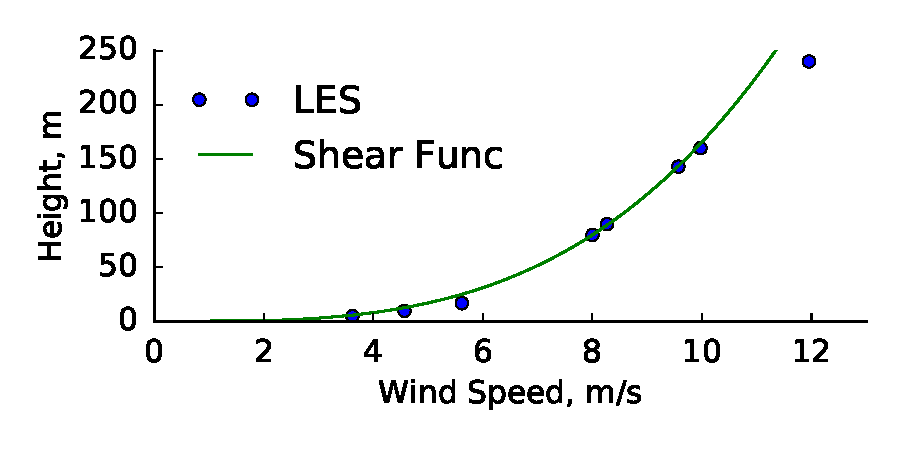
\includegraphics[width=0.75\textwidth]{final_images/shear_fit.pdf}
	\caption{The calculated wind speed using the power law (\cref{eq:shear}) with shear exponent $\psi=0.31$ compared with the values obtained from the LES precursor. The reference values used were a height of 80 m with a wind speed of 8 m/s}
	\label{fig:shear_fit}
\end{figure}
%

The results of the model changes discussed above can be seen in \cref{fig:model_contours}. These changes make the model continuous throughout the domain and differentiable everywhere except at the exact turbine location. With a separation constraint in place, the probability of turbines landing exactly on top of each other is extremely small, as noted in \cite{thomas2017}. While the linear interpolation makes very little attempt to be physically accurate in the near wake, the accuracy of the model for AEP calculation purposes should be unaffected since turbines will almost never be placed close enough together to be in the linear interpolation region in a final design. If greater accuracy is desired in the near wake, it would be feasible to use the linear interpolation during optimization and then switch to a more accurate near wake model for final calculations, such as the one proposed in \cite{keane2016}.

\begin{figure}[ht]
	\centering
	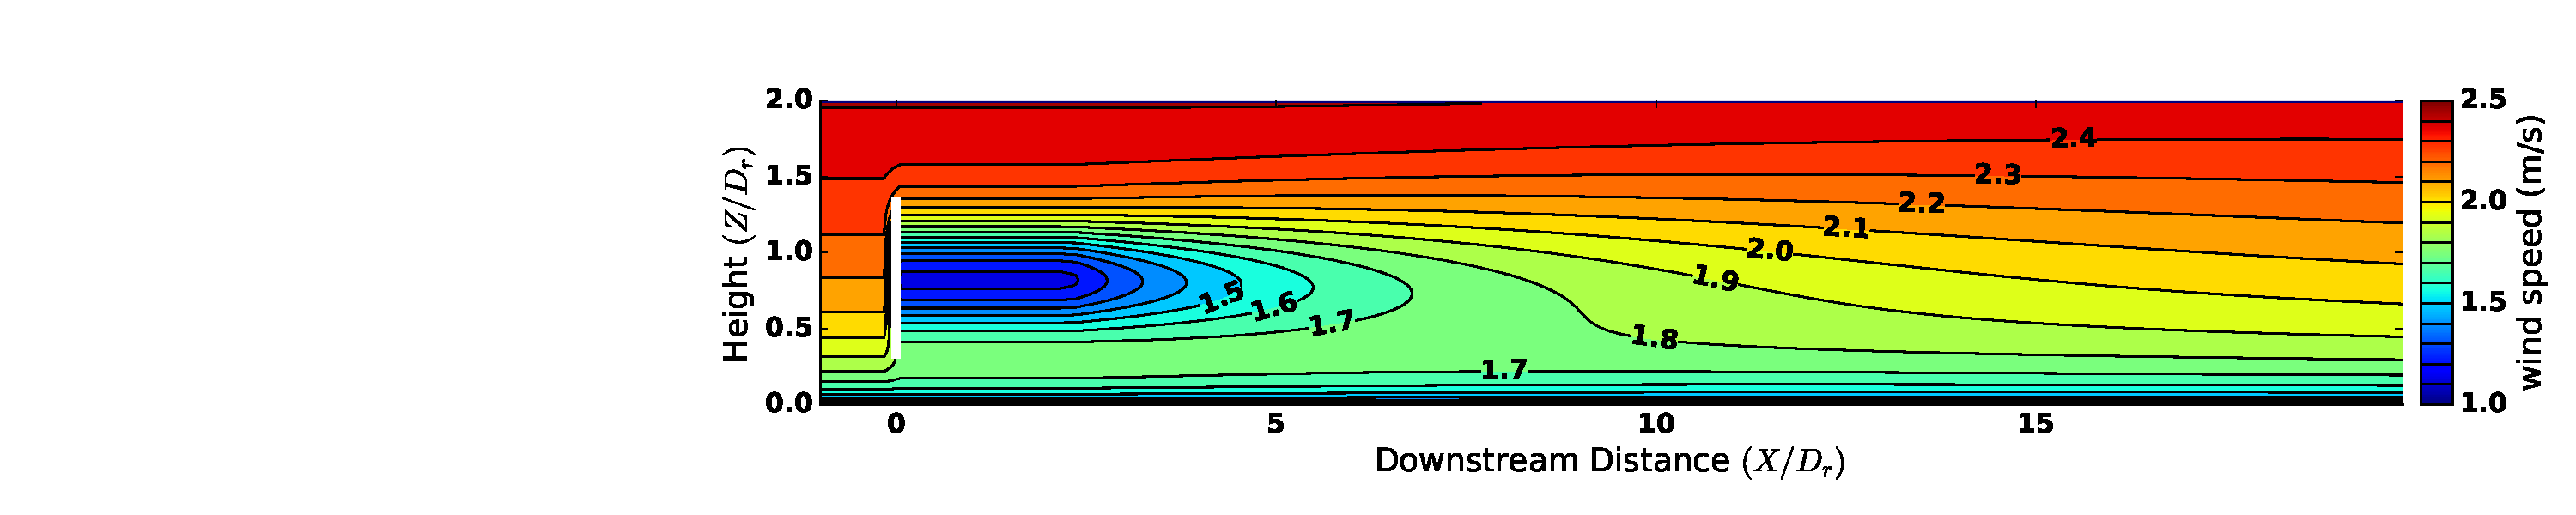
\includegraphics[width=0.75\textwidth, trim={18.5cm 1cm 4.cm 1cm}]{final_images/model_contours_vertical.pdf}
	\caption{Bastankhah and Port\'{e}-Agel wake model with the added linear interpolation for the near wake and shear model. The white line represents the turbine rotor. This figure was included for comparison with figure 6 of Bastankhah and Port\'{e}-Agel (2014) \cite{bastankhah2014}, and so model values were chosen accordingly. We used a shear exponent of 0.15 for this figure.}
	\label{fig:model_contours}
\end{figure}\todo{redo contour figure}


\subsection{Wind Farm Model}
\todo{include mention of thrust and power curves used and citation}
Niayifar and Port\'{e}-Agel proposed a wind farm model that used the Bastankhah and Port\'{e}-Agel model as published in 2014 \cite{bastankhah2014} for calculating the wind speed in the wakes \cite{niayifar2015, niayifar2016}. We applied the same wind farm model to the 2016 version of the Bastankhah and Port\'{e}-Agel model, with some variation as discussed in the following sections.
% However, due to changes made to the Bastankhah and Port\'{e}-Agel wake model published in 2016 \cite{bastankhah2016}, along with the needs of gradient-based optimization, not all of the proposals made by Niayifar and Port\'{e}-Agel in their 2016 paper can be used. This section will discuss which aspects of the Niayifar and Port\'{e}-Agel model that were and were not used in our system.
\subsubsection{Wake Combination}
Niayifar and Port\'{e}-Agel found the most accurate method of wake combination to be a linear interpolation that uses the inflow velocity of the upstream turbine as in \cref{eq:wake-comb-lin}. 
%
\begin{equation}\label{eq:wake-comb-lin}
	U_j = U_\infty - \sum_i (U_i - U_{i,j})
\end{equation}
%
Where $U_j$ is the inflow velocity at the turbine or point of interest, $U_i$ is the inflow velocity of upstream turbine $i$, $U_{i,j}$ is the wind speed that would exist at turbine or point $j$ if only turbine $i$ were accounted for, and $U_{\infty}$ is the freestream velocity. Our tests of the accuracy of various wake combination methods also found this method to be the most accurate. However, for the upstream turbine velocity to be used, the inflow velocity of the turbines must be calculated in order from upstream to downstream. We used the heapsort algorithm to obtain a sorted index list of the turbines prior to solving the system for each wind direction. Using the sorted index list allowed turbine sorting without over complicating the gradients of the system.

\subsubsection{Turbulence Intensity}
Niayifar and Port\'{e}-Agel calculated local turbulence intensity using the model presented by Crespo and Hern\'{a}ndez in \cite{crespo1996}. The local turbulence intensity is then applied to the Bastankhah and Port\'{e}-Agel model through an empirical model for calculating the wake expansion coefficient as shown in \cref{eq:ti_npa} \cite{niayifar2016}
 %
 \begin{equation} \label{eq:ti_npa}
 	k^* = 0.3837*I + 0.003678
 \end{equation}
%
Where $I$ is the turbulence intensity. This model is only valid for turbulence intensity values between 0.065 and 0.15. While the initial Bastankhah and Port\'{e}-Agel wake model, the wake model that the farm model presented by Niayifar and Port\'{e}-Agel is based on, does not include turbulence intensity \cite{bastankhah2014}, turbulence intensity was included by Bastankhah and Port\'{e}-Agel in their 2016 publication \cite{bastankhah2016}. We used the same turbulence intensity for the Bastankhah and Port\'{e}-Agel 2016 wake model as was used for the Niayifar and Port\'{e}-Agel wind farm model. Three different approaches to calculating turbulence intensity were employed at various points in the optimization process. (1) local turbulence intensity with a hard maximum function as done by Niayifar and Port\'{e}-Agel \cite{niayifar2016}, (2) local turbulence intensity with a smooth maximum function, and (3) ambient turbulence intensity only.

Local turbulence intensity with a hard maximum function as done by Niayifar and Port\'{e}-Agel \cite{niayifar2016} includes the use of a hard maximum function. The algorithm for calculating local turbulence intensity using the hard maximum function is given in \cref{alg:ti}. In our code implementation, we combined the nested loops used for the velocity and turbulence intensity calculations. 

Because the hard max creates discontinuites in the model and is not differentiable, we used a smooth maximum function during optimization. The smooth maximum function we used is shown in \cref{eq:smoothmax1,eq:smoothmax2,eq:smoothmax3} and is derived from the LogSumExp (LSE) function \cite{cook}.
%
\begin{equation}\label{eq:smoothmax1}
    t_{max} = \min(t_1, t_2)
\end{equation}
\begin{equation}\label{eq:smoothmax2}
    t_{min} = \max(t_1, t_2)
\end{equation}
\begin{equation}\label{eq:smoothmax3}
   \text{smoothmax}(t_{max},t_{min},s) = \frac{\ln(1+\exp(s(t_{min}-t_{max})))+s t_{max}}{s}
\end{equation}
%
where $s$ controls the smoothness of the transition between terms and influences the error of the calculation, $t_{max}$ and $t_{min}$ represent the respective maximum and minimum of the two values being compared, and $t_{smax}$ is the result of the smooth max function. In calculating local turbulence intensity, \cref{eq:smoothmax3} is applied as in  \cref{eq:maxti}
%
\begin{equation}\label{eq:maxti}
    I_{+_j} = \text{smoothmax}{\bigg(\frac{I_{+_{ij}}A_{w_{ij}}}{A_{r_j}}\bigg)}
\end{equation}
%
where $A_{w_{ij}$ is the area of the wake of turbine $i$ at the downstream location of turbine $j$, $A_{r_j}$ is the area of the the rotor of turbine $j$, and $I_{+_{ij}}$ is the added turbulence intensity from turbine $i$ at the downstream location of turbine $j$. The total turbulence intensity is then calculated using \cref{eq:ti_at_turb}
%
\begin{equation}\label{eq:ti_at_turb}
    I_j = \sqrt{I_0^2+I_{+_j}^2}
\end{equation}
%
\todo{consider making it more clear that only two values are compared in the smooth max at a time}
The maximum error of \cref{eq:smoothmax3} occurs when $t_{min} = t_{max}$, and can be calculated as $Error_{max} = \ln{(2)}/s$. To keep the error from the smooth max below 0.001, or about 1\% of the total turbulence intensity, we set $s=700$.

% Using \cref{eq:ti_npa} in the updated wake model would cause the effects of turbulence intensity to be included twice. We used \cref{eq:ti_npa} to estimate the initial $k^*$ only. Within the model itself, the ambient turbulence intensity only impacts the model through Bastankhah and Port\'{e}-Agel (2016) \cite{bastankhah2016} and local turbulence intensity is not calculated. 
%
%Jen changes
% \begin{algorithm}
% 	\caption{Turbulence Intensity Calculation}
%    \label{alg:ti}
%    \begin{algorithmic}
%    \Ensure Turbines are sorted by relative downstream position
%      \For{$j =  1...N$} \Comment{Downstream turbines}
%    	\State $I_{+,j} \gets 0$
%          \For{$i =  1...N$} \Comment{Upstream turbines}
%          	\State $\Delta X \gets x_j - x_i$ 
%          	\If{$\Delta X > 0$}
%                \State $\beta \gets 0.5((1+\sqrt{1-C_{T,i}})/\sqrt{1-C_{T,i}})$
%                \State $\epsilon \gets 0.2 \sqrt{\beta}$
%                \State $\sigma = k_i^*\Delta X+D_{r,i}\epsilon$
%                \State $D_w \gets 4\sigma$
%                \State $A_{w,i,j} \gets$ Wake overlap area of wake $i$ and rotor $j$ \Comment{Circular wake}
%                \State $A_{r,j} \gets \pi D_{r,j}^2/4$ \Comment{Rotor-swept area}
%                \State $I_{+,i,j} \gets 0.73 a_{i}^{0.8325} I_{0,i}^{0.0325} (\Delta X/D_{r,i})^{-0.32}$
%                \State $I_{+,j} \gets \max{((I_{+,i,j}A_{w,i,j}/A_{r,j}), (I_{+,i-1}))}$ \Comment{Discontinuity here}
%         	\EndIf
%         \EndFor
%         \State $I_{0,j} \gets \sqrt{I^2 + I_{+,j}^2}$
%         \State $k_j^* \gets 0.3837I_{0,j}+0.003678 $ \Comment{To be used in the BPA wake model}
%      \EndFor
%    \end{algorithmic}    
% \end{algorithm}
% 
\todo{need to address optimizing without local TI and then with}
\todo{check the algorithm and update as needed}
\begin{algorithm} \label{alg:ti}
	\caption{Turbulence Intensity Calculation (for more information, see \cite{niayifar2016})}
   \label{alg:ti}
   \begin{algorithmic}
   \Ensure Turbines are sorted by relative downstream position
     \For{$j =  1...N$} \Comment{Downstream turbines}
   	% \State $I_j \gets I_0$ \Comment{Initialize to free-stream turbulence value}
    \State $A_{r_j} \gets \frac{1}{4}\pi D_{r_j}^2$ \Comment{Rotor swept area of turbine $j$}
    \State $I_{+_j} \gets 0$
         \For{$i =  1...N$} \Comment{Upstream turbines}
         	\State $\Delta X \gets x_j - x_i$ \Comment{Turbine separation distance}
         	\If{$\Delta X > 0$}
               \State $\beta \gets 0.5((1+\sqrt{1-C_{T_i}})/\sqrt{1-C_{T_i}})$
               \State $\epsilon \gets 0.2 \sqrt{\beta}$
               \State $\sigma = k_i^*\Delta X+D_{r_i}\epsilon$
               \State $D_w \gets 4\sigma$
               \State $A_{w_{ij}} \gets$ Wake overlap area of wake $i$ and rotor $j$ \Comment{Assume circular wake}
               \If{$C_T_i > 0.96$}
                    \State $a_i \gets 0.143 + \sqrt{0.0203-0.6427(0.889 - C_T_i)}$ \Comment{Glauert correction\cite{gebraad2017-max-aep}}
               \Else
                   \State $a_i \gets  \frac{1}{2}(1-\sqrt{1-C_{T_i}})$
               \EndIf
               
               \State $I_{+_{ij}} \gets 0.73 a_{i}^{0.8325} I_i^{0.0325} (\Delta X/D_{r_i})^{-0.32}$
               \State $I_{+_j} \gets \max{(I_{+_{ij}}A_{w_{ij}}/A_{r_j}, I_{+_j})}$ \Comment{We used \cref{eq:smoothmax3} during the final optimization}
        	\EndIf
        \EndFor
        \State $I_j \gets \sqrt{I_{0}^2 + I_{+_j}^2}$ \Comment{Directly influenced by only one upstream turbine}
        \State $k_j^* \gets 0.3837I_j+0.003678 $ \Comment{To be used in the wake model calculations}
     \EndFor
   \end{algorithmic}    
\end{algorithm}

\subsubsection{Sampling Over the Rotor-Swept Area}
For efficiency during optimization, we approximated the effective velocity of each wind turbine by using a single sampling point located at the rotor hub \todo{expand rotor sampling discussion}
%four sampling points located to the right, left, top, and bottom of the rotor hub and spaced at 69$\%$ of the rotor diameter from the center of the hub position as shown in \cref{fig:sampling_locs}(a). This location corresponds to the approximate radial position of the highest loads on the turbine blades
%according to Blade Element Momentum (BEM) theory 
as shown in \cref{fig:sampling_locs}(b).

\begin{figure}[ht]
	\centering
	\subfigure[]{
		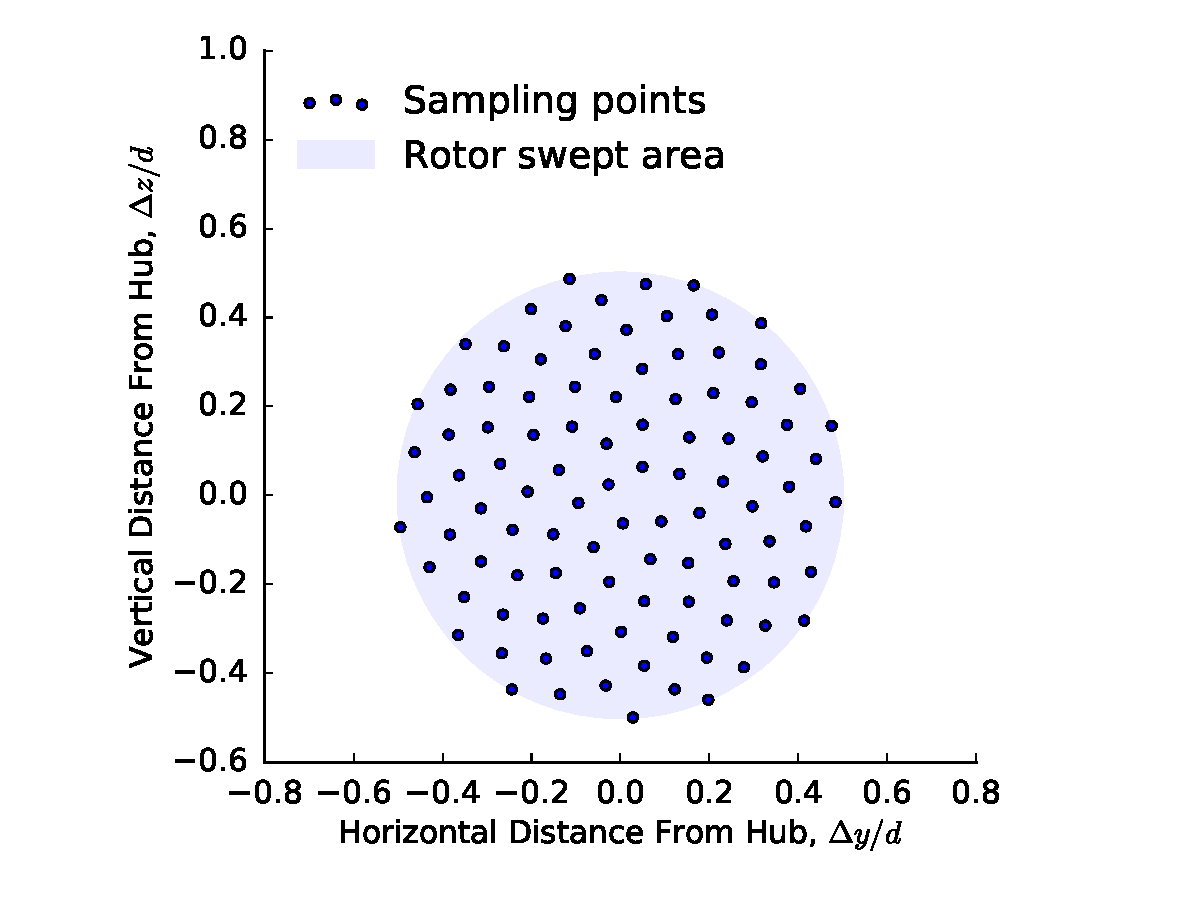
\includegraphics[width=0.48\textwidth, trim={0cm 0cm 0cm 0cm}]{final_images/one_hundred_sampling_points.pdf}
	}
    \subfigure[]{
		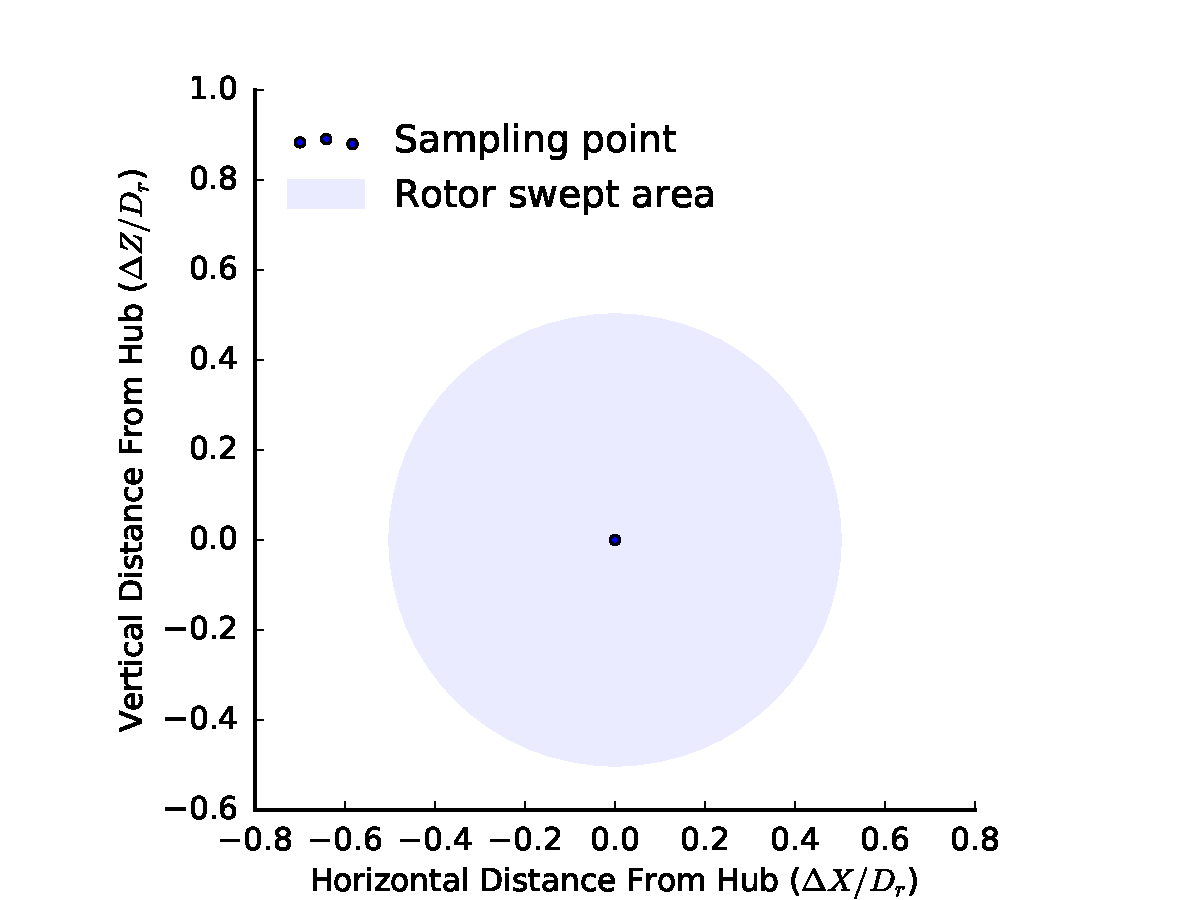
\includegraphics[width=0.48\textwidth, trim={0cm 0cm 0cm 0cm}]{final_images/one_sampling_point.pdf}
	}
% 	\subfigure[]{
% 		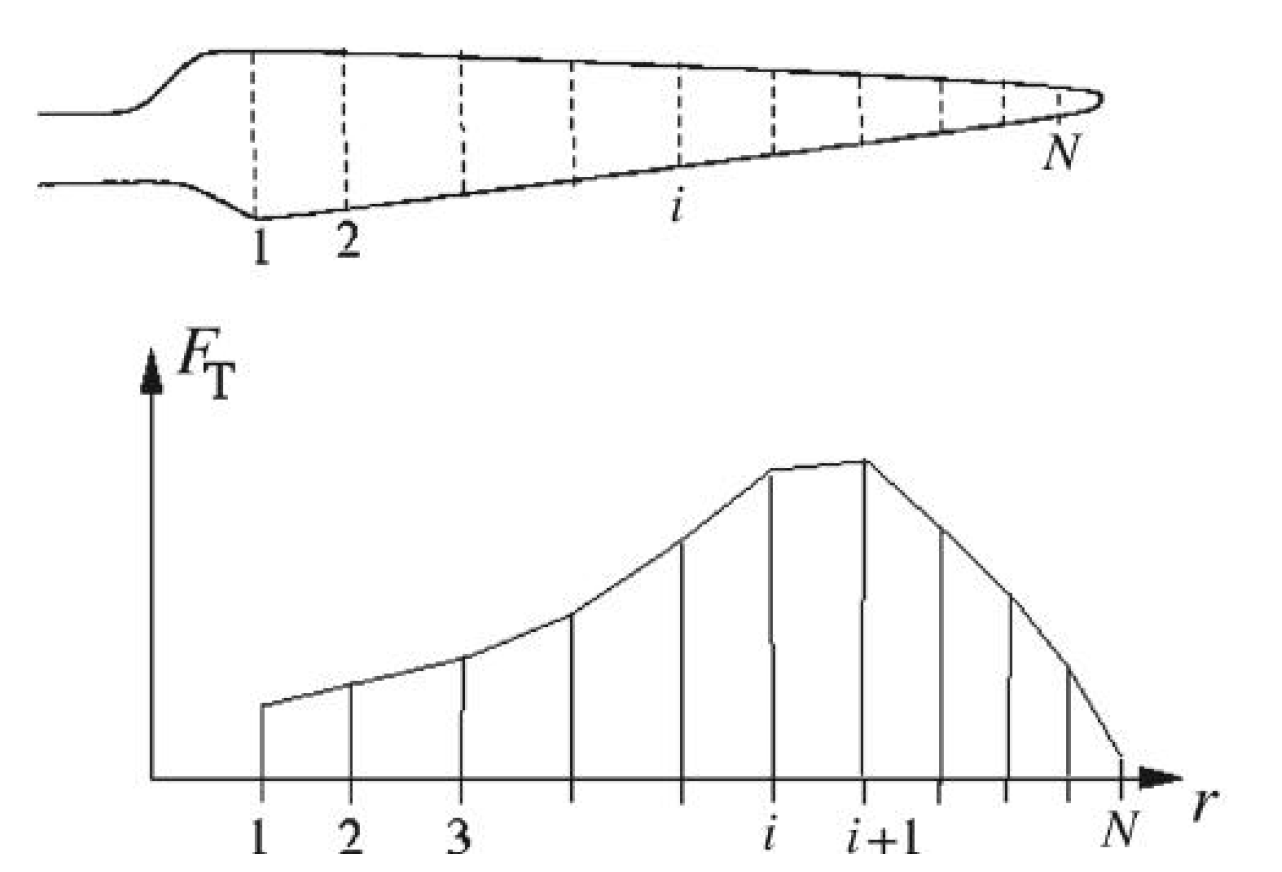
\includegraphics[width=0.43\textwidth, trim={0cm -1cm 0cm 0cm}]{final_images/bem_distribution.png}
% 	}
	\caption{(a) Dense sampling used to approximate effective hub velocity for LES comparisons. (b) Location of sampling point for approximating effective hub velocity during optimization.}
	\label{fig:sampling_locs}
\end{figure}

\subsubsection{Reproducing Previous Results}
Using our implementation of the models just described, we were able to reproduce the results of Niayifar and Port\'{e}-Agel \cite{niayifar2016} as shown in \cref{fig:power_line,fig:power_direction}. For the optimization we used the definition of the power coefficient to calculate power as done in \cite{gebraad2014}. \todo{expand discussion of results duplication} \todo{include something about using WEC}

\begin{figure}[ht]
	\centering
	\subfigure[]{
		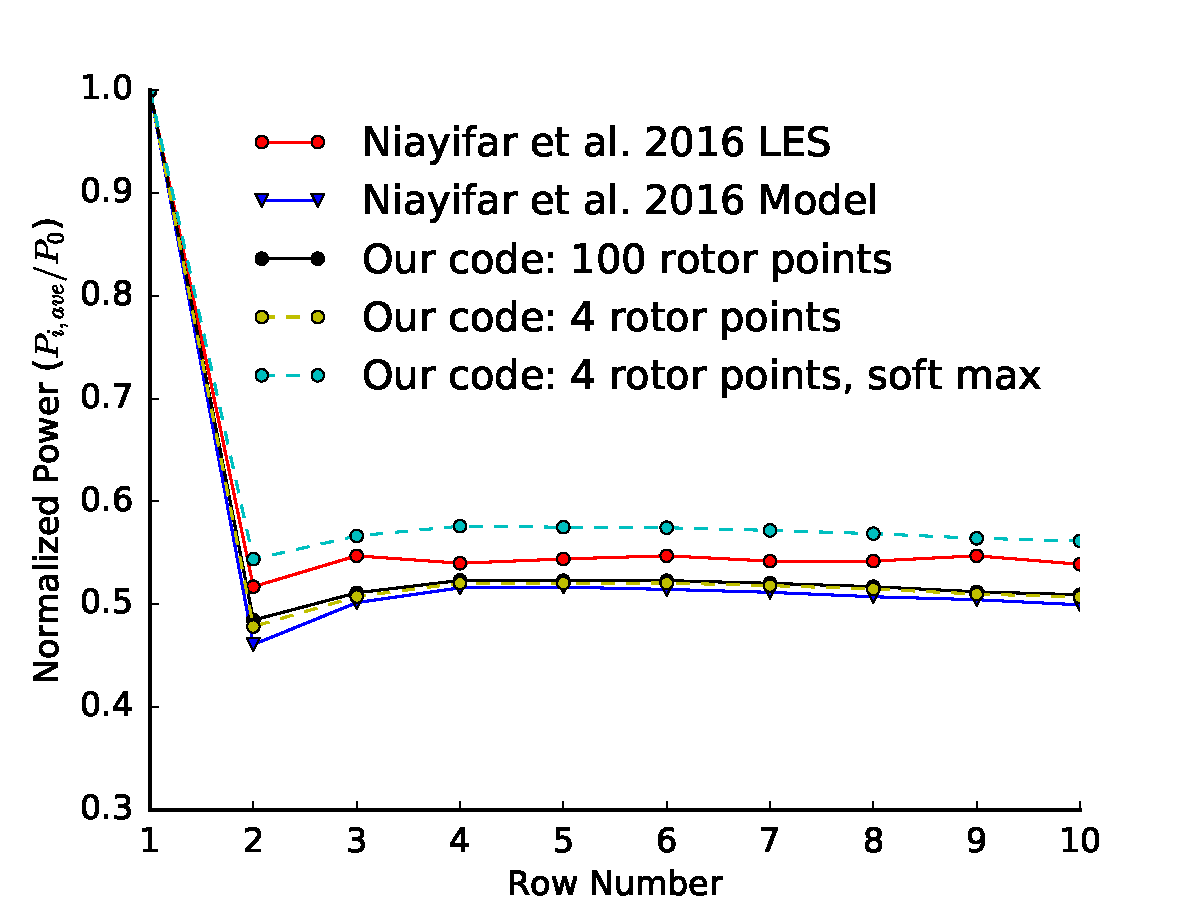
\includegraphics[width=0.48\textwidth, trim={0cm 0cm 0cm 0cm}]{final_images/power_row_2014.pdf}
	}
	\subfigure[]{
		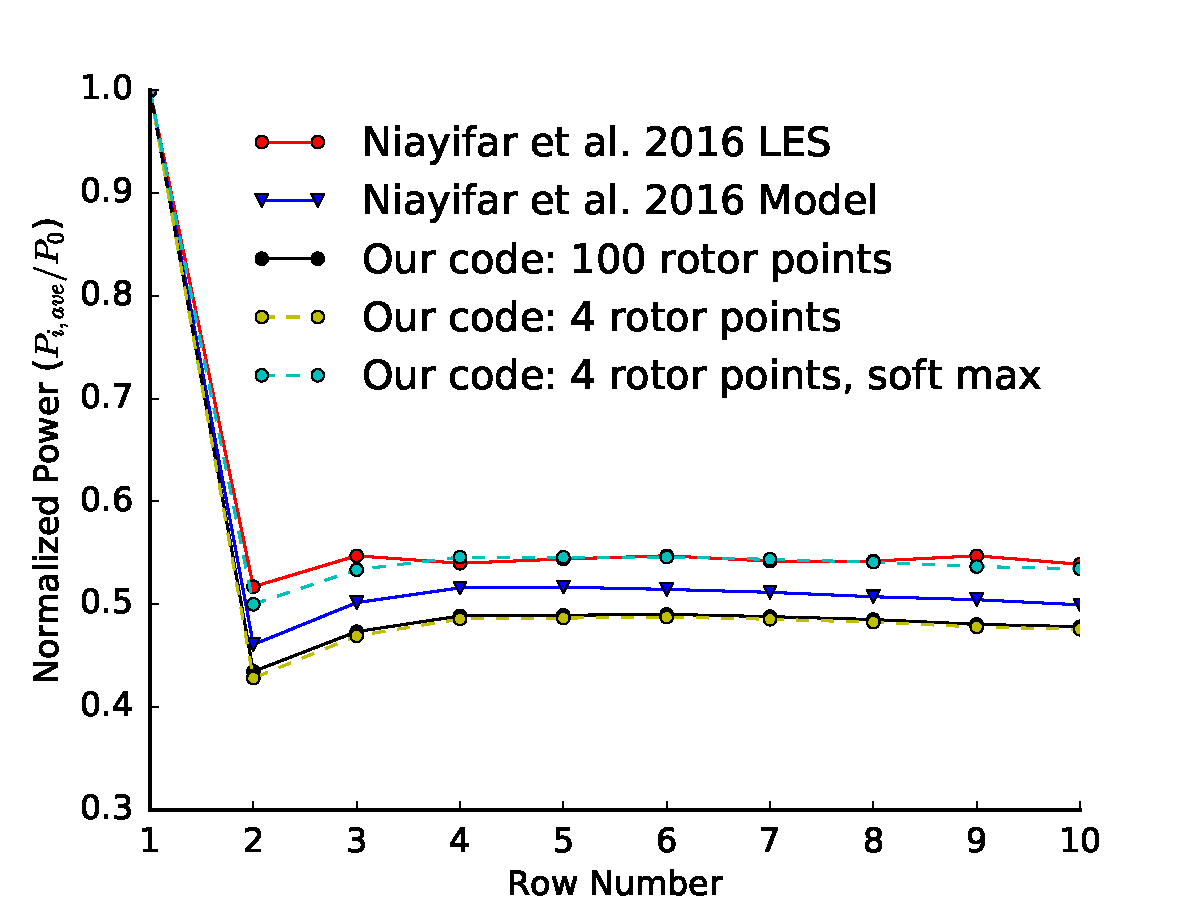
\includegraphics[width=0.48\textwidth, trim={0cm 0cm 0cm 0cm}]{final_images/power_row_2016.pdf}
	}
	\caption{Averaged power of turbines in columns two, three, and four of the Horns Rev wind farm by turbine row. Data from \cite{niayifar2016}. (a) Comparing our implementation of the 2014 version of the Bastankhah and Port\'{e}-Agel wake model. (b) Comparing our implementation of the 2016 version of the Bastankhah and Port\'{e}-Agel wake model.}
	\label{fig:power_line}
\end{figure}

\begin{figure}[ht]
	\centering
	\subfigure[]{
		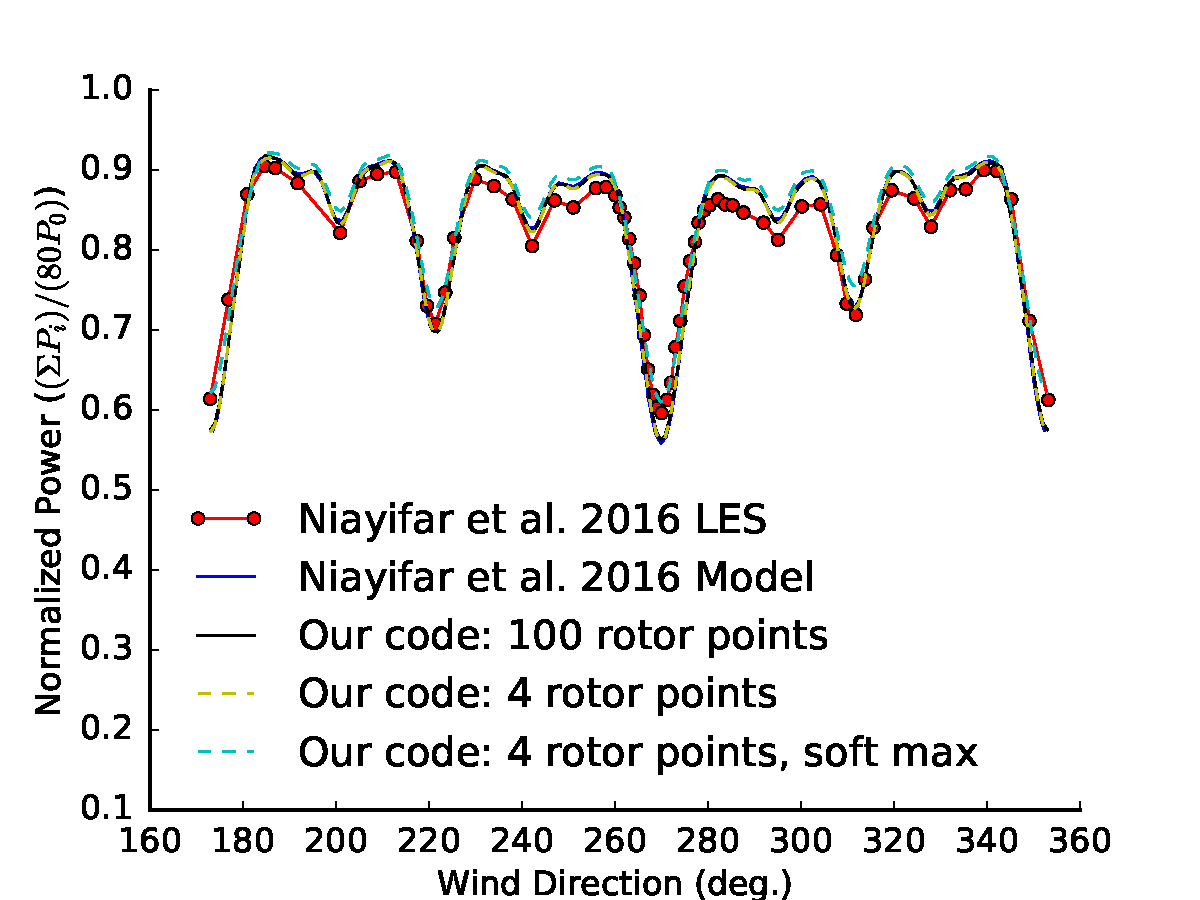
\includegraphics[width=0.48\textwidth, trim={0cm 0cm 0cm 0cm}]{final_images/power_direction_2014.pdf}
	}
	\subfigure[]{
		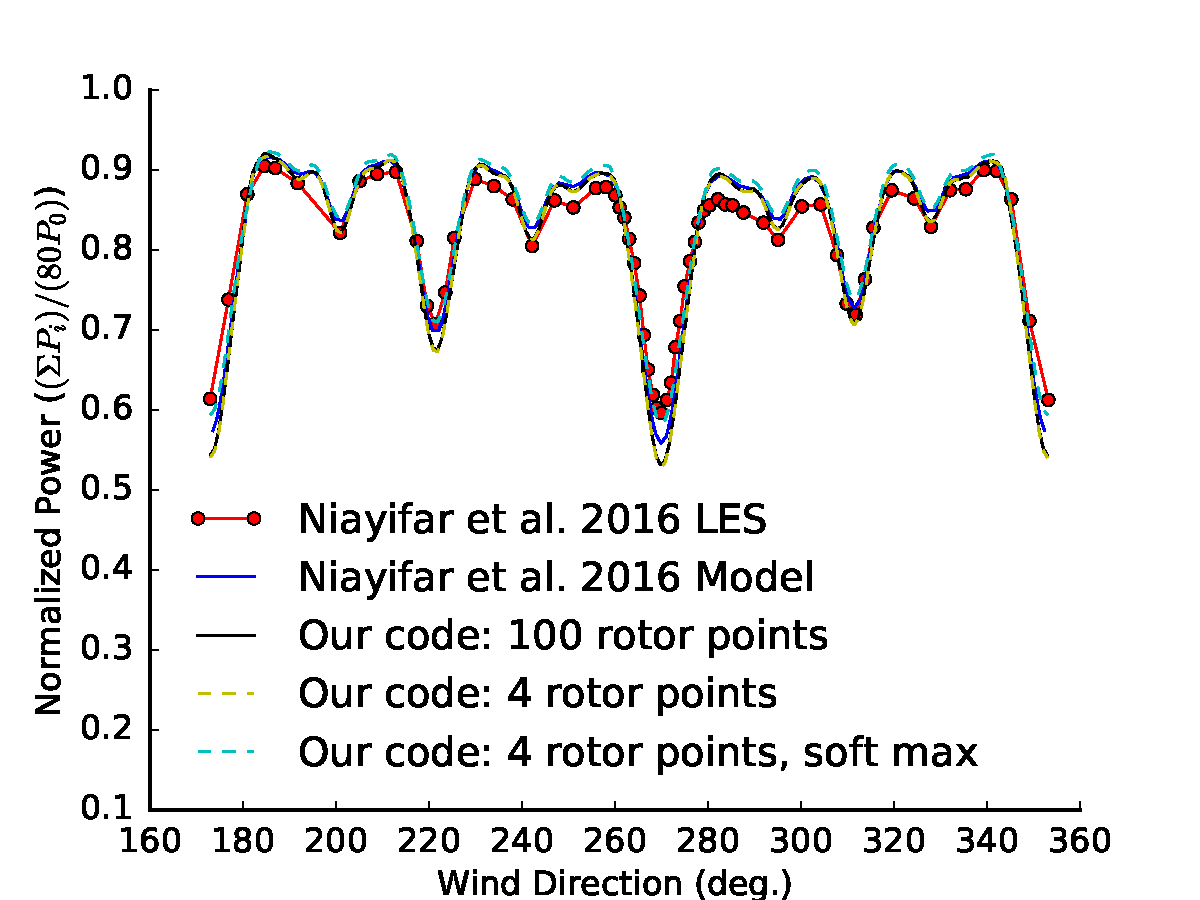
\includegraphics[width=0.48\textwidth, trim={0cm 0cm 0cm 0cm}]{final_images/power_direction_2016.pdf}
	}
	\caption{Power by direction. Data from \cite{niayifar2016}. (a) Comparing our implementation of the 2014 version of the Bastankhah and Port\'{e}-Agel wake model. (b) Comparing our implementation of the 2016 version of the Bastankhah and Port\'{e}-Agel wake model.}
	
	\label{fig:power_direction}
\end{figure}

\subsection{Test Case}

For the LES validation, we used the NREL 5-MW reference turbine \cite{jonkman2009}. Our test wind farm was constrained by the domain of the LES simulation precursor. We limited the LES simulation to an area 5 km square to keep necessary computational resources to a reasonable level. In order to avoid edge effects in the simulation, we needed at least 0.5 km between the edge of wind farm and the edge of the simulation space. To limit the computational cost, we used only a single wind direction and rotated the wind turbine locations within the simulation space to calculate the power production in different directions so that a single pre-cursor could be used. The resulting available space for the wind farm was a circle with a 2 km radius in the middle of the simulation space. Within the resulting circular region, we placed as many turbines as possible in a concentric circular pattern with a minimum allowable distance between turbines of 5 times the rotor diameter. The resulting layout is shown in \cref{fig:starting-layout}.    

\begin{figure}[ht]
	\centering
	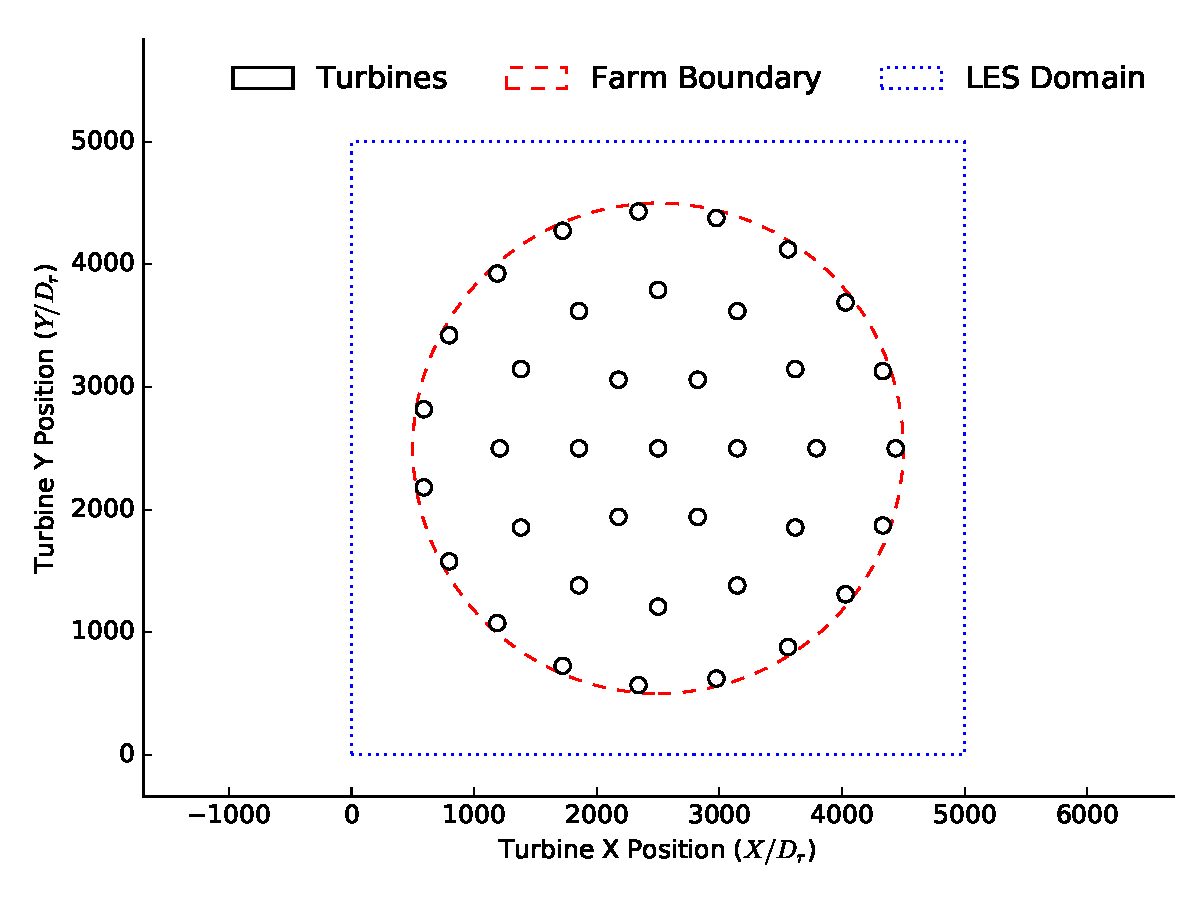
\includegraphics[width=0.75\textwidth]{final_images/round_farm_38Turbines_5DSpacing.pdf}
	\caption{Base case wind farm layout. The circles marking turbine locations are to scale, with diameters equal to the rotor diameter.}
	\label{fig:starting-layout}
\end{figure}

For the wind frequencies, we chose to use the Nantucket wind rose \cite{wrcc2017} %was selected as an approximation of the wind rose of the new Bay State Wind farm proposed for development off the coast of Massachusetts \cite{baystate2017}
. From this wind rose, 12 directions were selected by binning every 3 directions from the original wind rose starting with wind from the North. The original and final wind roses can be seen in \cref{fig:windrose}.

\begin{figure}[ht]
	\centering
	\subfigure[]{
		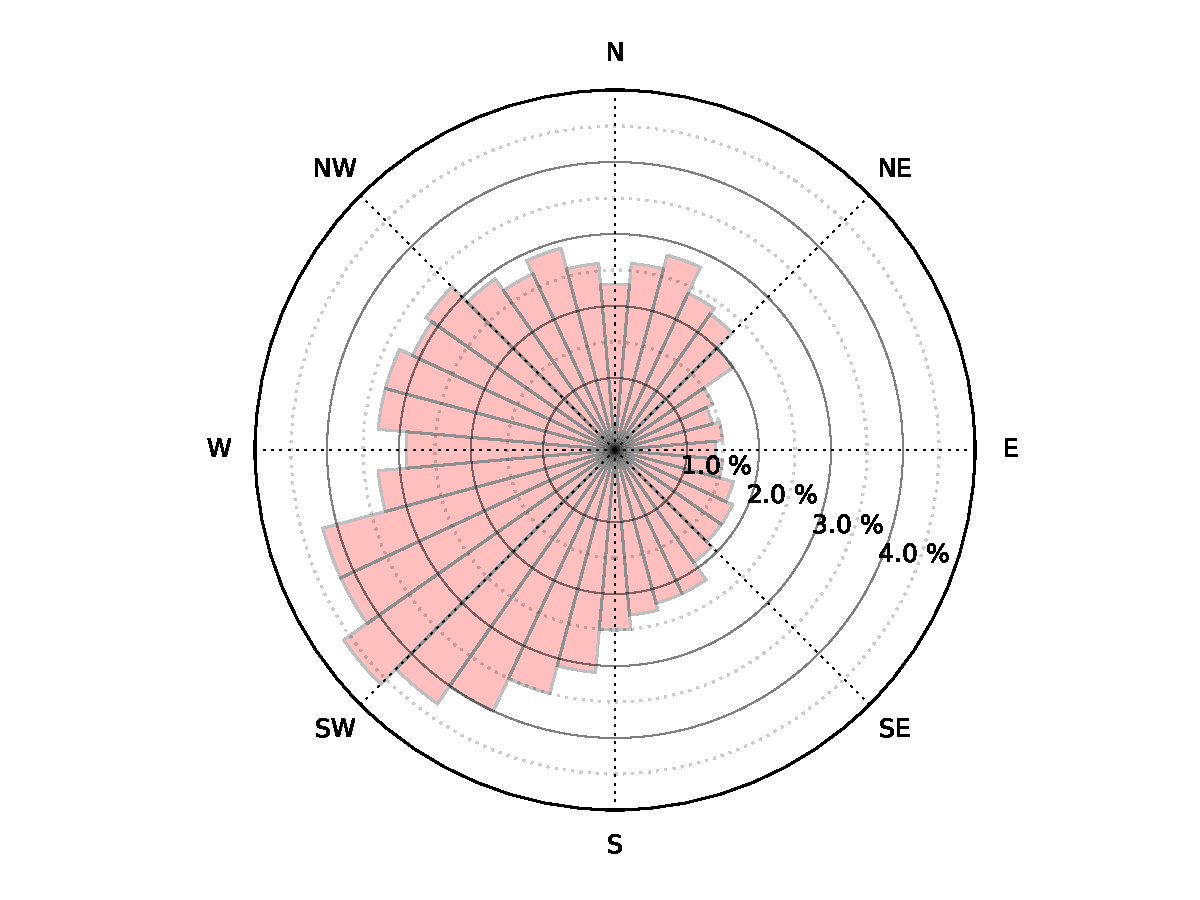
\includegraphics[width=0.48\textwidth, trim={3.25cm 0cm 3.25cm 0cm}]{final_images/windrose_full.pdf}
	}
	\subfigure[]{
		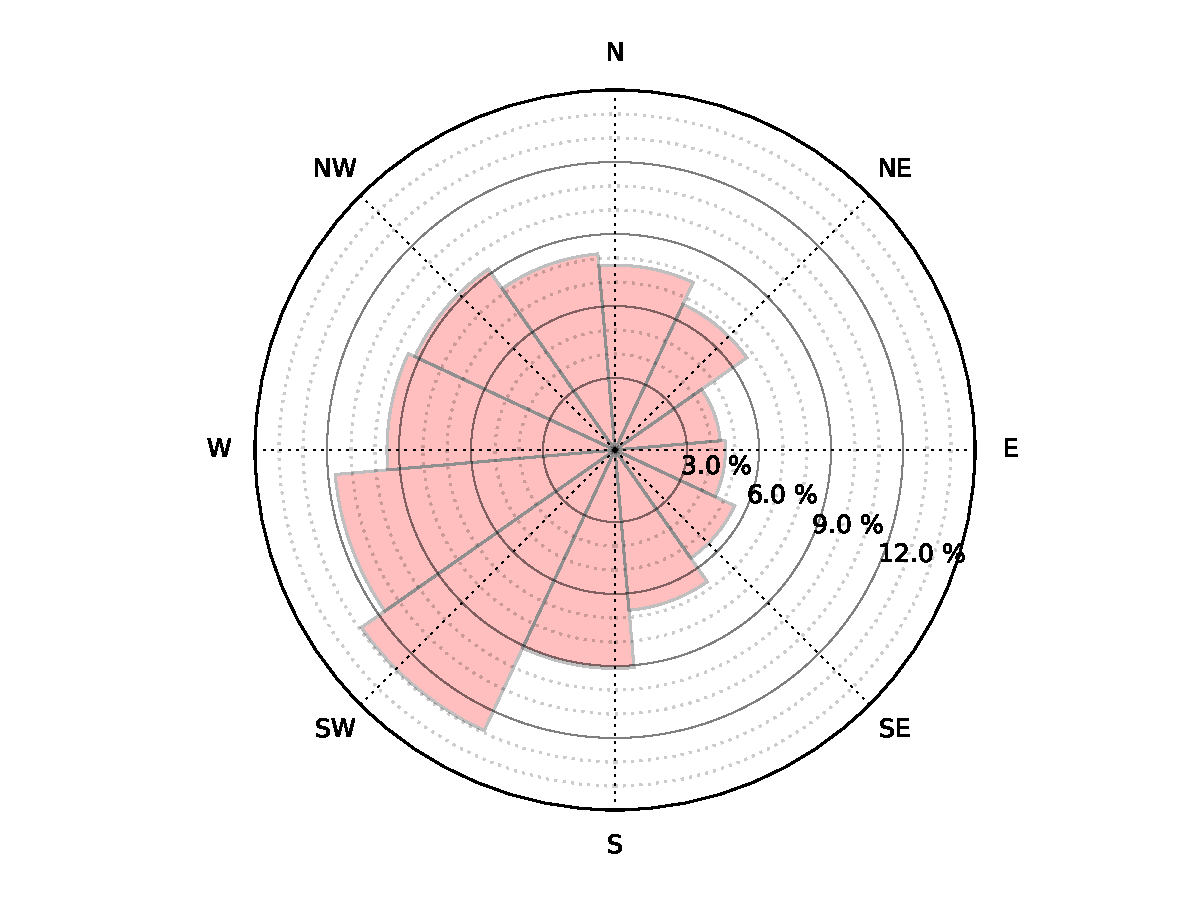
\includegraphics[width=0.48\textwidth, trim={3.25cm 0cm 3.25cm 0cm}]{final_images/windrose_les.pdf}
	}
	\caption{(a) Nantucket frequency windrose \cite{wrcc2017}. (b) Nantucket frequency windrose binned into 12 directions}
	\label{fig:windrose}
\end{figure}

\subsection{Optimization}

We optimized the layout using Annual Energy Production (AEP) as the objective. The optimization problem was formulated as
%
\begin{equation}
	\label{e:objective}
	\begin{aligned} [b]
	\underset{x_i,y_i}{\textrm{maximize}} \quad & AEP(x_i,y_i,)~~i=1...38\\
	\textrm{subject to} \quad & S_{i,j} \geq 2\*D_{r}~~i,j=1...38~~i \neq j\\
	 & [x_c-x_i]^2+[y_c-y_i]^2 \leq r_{b}^2~~i=1...38\\
	\end{aligned}
\end{equation}
%
Where $(x_i,y_i)$ is the position of each turbine $i$, $S_{i,j}$ represents the separation distance between each pair of turbines $i$ and $j$, $D_{r}$ is the rotor diameter, $(x_c,y_c)$ is the location of the center of the wind farm, and $r_b$ is the radius of the wind farm boundary.

The optimization problem was built in OpenMDAO, a Multidisciplinary Design Analysis and Optimization platform  \cite{gray2010_OpenMDAO}. Gradients of the wake model were obtained using Tapenade, an algorithmic differentiation tool \cite{tapenade2013}. Gradients of all other system components were derived by hand. The final system gradients were combined by OpenMDAO. \todo{include ignoring inactive constraints?}

Once the problem was set up, it was scaled such that the gradients of both the objective function and constraints were close to order one. The final problem was then solved using SNOPT (Sparse Nonlinear OPTimizer), a gradient-based optimization algorithm that uses a sequential quadratic programming approach.  SNOPT was used in this case because it is well suited to non-linear problems with high dimensionality \cite{gill2005}. The optimization was performed from the base case layout and 199 random layouts.  

\subsection{LES}
\todo{where does the following LES refs go? Also seems like wrong TI} The grid cells have a 10\,m spacing in the $x$, $y$, and $z$ directions.  The simulation is run as a neutral boundary layer with 5.6\% turbulence intensity and 8\,m/s at hub height.
% Precursor?

% Layout?

% Rotation?

\subsection{Comparing LES and Model Results}
% Comparison Approach

% Directional Power

% AEP

\section{Results and Discussion}

\subsection{Base Case Layout} \todo{fill in this section with LES comparison figures and discussion}
The 200 starting layouts' AEP is provided in \cref{fig:opt-distribution}.

\subsection{Optimized Layout} \todo{re-outline this section}

\todo{re-write this section} The 200 starting layouts exhibited a distribution of results demonstrating the highly multi-modal nature of the WFLOP design space. The distribution of the optimization results can be seen in \cref{fig:opt-distribution}.

\begin{figure}[ht]
	\centering
	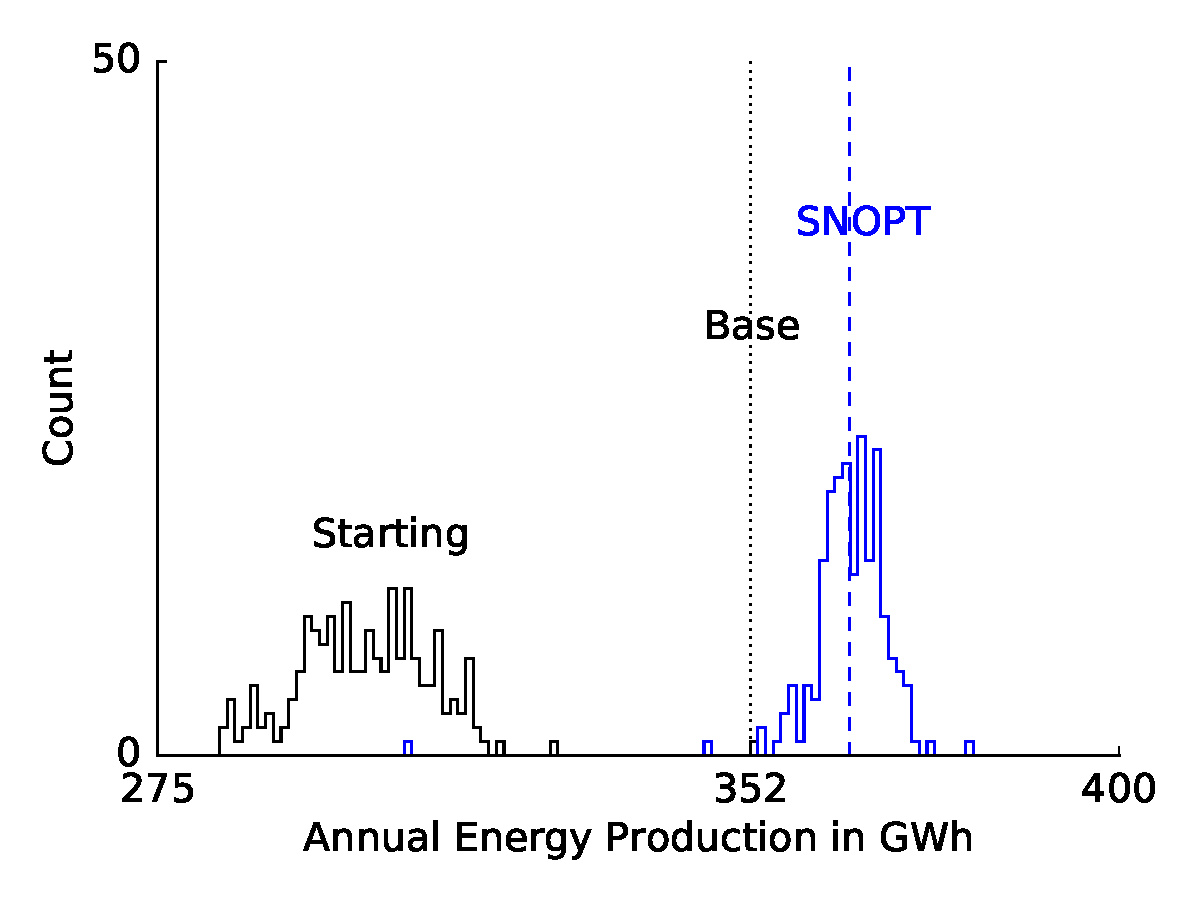
\includegraphics[width=0.75\textwidth]{final_images/orig_dist.pdf}
	\caption{Distribution of AEP results from the 200 starting layouts. The dotted line labeled as Base indicates the AEP of the base case layout.}
	\label{fig:opt-distribution}
\end{figure}

Of the 200 starting layouts, the planned starting layout (shown in \cref{fig:starting-layout}) resulted in the highest AEP. 

\todo{outline LES methods and R&D sections}
%The final layout with the highest AEP is shown in \cref{fig:final-layout}.

% \begin{figure}[ht]
% 	\centering
% 	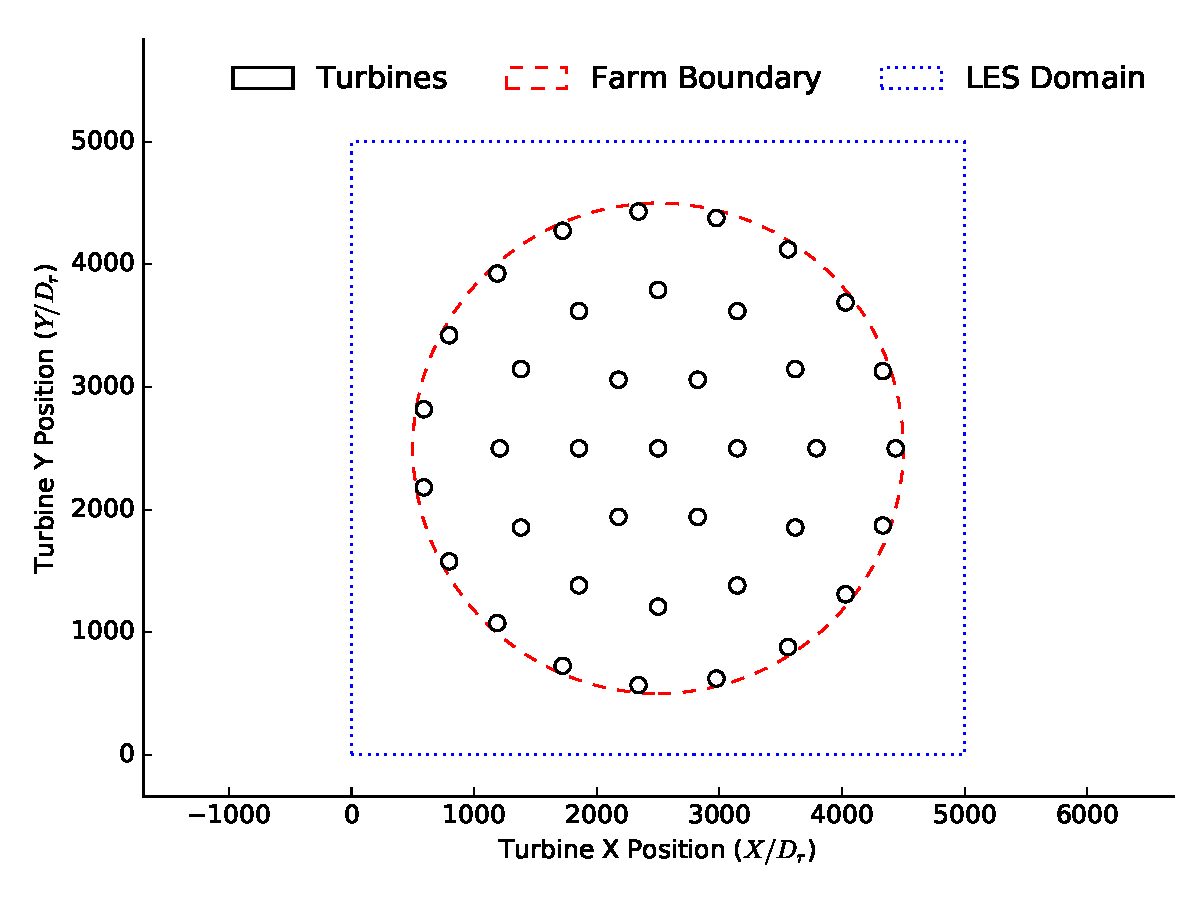
\includegraphics[width=0.75\textwidth]{final_images/round_farm_38Turbines_5DSpacing.pdf}
% 	\caption{Final optimized layout with the highest AEP. Obtained using the starting positions shown in \cref{fig:starting-layout}}
% 	\label{fig:final-layout}
% \end{figure}

% \subsubsection{Simplified Modeling}

% \subsubsection{LES Modeling}

% \subsubsection{Comparison}

% \subsection{Expected Results}
% We will run the each of the 12 wind directions using LES for both the base layout and the final optimized layout. To validate the results, we will compare the percent improvement in: total AEP,  directional power for each direction, and the power production of each individual turbine in each direction. The optimization results will be considered validated if the relative change from base to optimized layout at each level of granularity (i.e. AEP, direction, and turbine) for LES and the Bastankhah and Port\'{e}-Agel wake model are similarly significant and follow similar trends. We may also be able to determine how much of the improvement is real. We plan to provide bar charts, results tables, and other figures as appropriate.

%cases you plan to run, how you plan to use LES, the metrics you will use to compare (and what would be considered "validated"), etc.
% \section{Conclusion}
% This validation study will help us and other researchers understand how much of the improvement during optimization is real, and not an artifact of the models being used. This in turn will help us know how much improvement is needed based on simplified models to result in meaningful improvements to a real wind farm. 

\clearpage

\bibliographystyle{unsrt}
\bibliography{references/all_refs}
\end{document}